\chapter{Rappel : éléments de calcul vectoriel}
\section{Produit vectoriel}
	\subsection{Définition}
		\label{sec:def-prodvect}
		\begin{definition}
		Soient \vect{u} et \vect{v} deux vecteurs. On notera $\vect{u}\wedge\vect{v}$ le produit vectoriel de \vect{u} et \vect{v}.
		
%	\subsection{Propriétés}
	Soit \vect{w} un vecteur tel que $\vect{u}\wedge\vect{v}=\vect{w}$. On a alors, par définition du produit vectoriel :
	\begin{itemize}
		\item $\vect{w}$ est orthogonal à $\vect{u}$ et $\vect{v}$,
		\item la base $(\vect{u},\vect{v},\vect{w})$ est directe\footnote{C'est-à-dire qu'elle respecte la règle dite \og des trois doigts de la main droite \fg{}.},
		\item $||\vect{w}||=||\vect{u}||\cdot||\vect{v}||\cdot|\sin(\vect{u},\vect{v})|$.
	\end{itemize}
	\end{definition}
La figure~\ref{fig:produit-vect} illustre ces propriétés.	
	
	\begin{figure}[htbp]
		\centering
		\tdplotsetmaincoords{70}{130}
		\begin{tikzpicture}[tdplot_main_coords,scale=3]
			\draw[,thick,-latex,red] (0,0,0) --(0.7,0,0) node[anchor=north east]{$\vect{u}$};
			\draw[,thick,-latex,blue] (0,0,0) --(0,1.4,0) node[anchor=west]{$\vect{v}$};
			\draw[,thick,-latex,green] (0,0,0) --(0,0,0.98) node[anchor=west]{$\vect{u}\wedge\vect{v}$};
			\tdplotdrawarc[,-stealth]{(0,0,0)}{0.3}{0}{90}{anchor=north}{+}	
			\tdplotsetrotatedcoords{0}{0}{0}
			\tdplotsetrotatedthetaplanecoords{0}	
			\tdplotdrawarc[tdplot_rotated_coords,-stealth]{(0,0,0)}{0.3}{0}{90}{anchor=east}{+}										
			\tdplotsetrotatedthetaplanecoords{90}	
			\tdplotdrawarc[tdplot_rotated_coords,stealth-]{(0,0,0)}{0.3}{0}{90}{anchor=west}{+}	
		\end{tikzpicture}
		\caption{Représentation 3D du produit vectoriel.}
		\label{fig:produit-vect}
	\end{figure}
	D'après la définition précédente, $\vect{u}\wedge\vect{v}=\vect{0}$ si et seulement si $\vect{u}$ et $\vect{v}$ sont colinéaires\footnote{Si l'un des vecteurs est nul, alors il est colinéaire à l'autre.}.
	
	\subsection{Propriétés}
	Le produit vectoriel respecte les propriétés suivantes :
	\begin{itemize}
		\item Il est distributif sur l'addition :
			\begin{equation}
				\left(\vect{u}+\vect{v}\right)\wedge\vect{w}=\vect{u}\wedge\vect{w}+\vect{v}\wedge\vect{w}
			\end{equation}
		\item Il est compatible avec la multiplication par un scalaire :
			\begin{equation}
				\left(\lambda\vect{u}\right)\wedge\vect{v}=\lambda\left(\vect{u}\wedge\vect{v}\right)
			\end{equation}
		\item Il est antisymétrique :
			\begin{equation}
				\vect{u}\wedge\vect{v}=-\vect{v}\wedge\vect{u}
			\end{equation}
	\end{itemize}
	
	\subsection{Calcul}
		Soient deux vecteurs \vect{u} et \vect{v} de coordonnées suivantes :
		\begin{equation}
			\vect{u}
			\left|
			\begin{array}{c}
				u_x\\
				u_y\\
				u_z\\
			\end{array}
			\right.
			\quad
			\text{et }
			\vect{v}
			\left|
			\begin{array}{c}
				v_x\\
				v_y\\
				v_z\\
			\end{array}
			\right.
			\,.		
		\end{equation}
Si $\vect{w}=\vect{u}\wedge\vect{v}$, on a alors :
\begin{equation}
			\vect{w}
			\left|
			\begin{array}{c}
				u_yv_z-v_yu_z\\
				u_zv_x-v_zu_x\\
				u_xv_y-v_xu_y\\
			\end{array}
			\right.
\end{equation}

\section{Extension : produit mixte}
	\subsection{Définition}
		\begin{definition}
			Soient \vect{u}, \vect{v} et \vect{w} trois vecteurs. On note $[\vect{u}, \vect{v}, \vect{w}]$ le scalaire, appelé produit mixte de \vect{u}, \vect{v} et \vect{w}, tel que :
			\begin{equation}
				[\vect{u}, \vect{v}, \vect{w}]=\left(\vect{u}\wedge\vect{v}\right)\cdot\vect{w}
			\end{equation}
			où $\cdot$ est le produit scalaire.
		\end{definition}
		
	\subsection{Propriétés}
		\label{sec:props-prodmixte}
		Outre ses propriétés de linéarité, qui découlent directement de celles du produit vectoriel, le produit mixte respecte les propriétés suivantes :
		\begin{itemize}
			\item Il est identique par permutation circulaire :
			\begin{equation}
				[\vect{u}, \vect{v}, \vect{w}]=[\vect{v}, \vect{w},\vect{u}]=[\vect{w},\vect{u}, \vect{v}]
			\end{equation}
			\item Il est anticommutatif :
			\begin{equation}
				[\vect{u}, \vect{v}, \vect{w}]=-[\vect{v},\vect{u},\vect{w}]=-[\vect{w},\vect{v}, \vect{u}]=-[\vect{u}, \vect{w}, \vect{v}]
			\end{equation}			
		\end{itemize}
		
		
\section{Torseur}
	\subsection{Champ de vecteurs équiprojectif}
On considère un champ de vecteur de l'espace $E$. On note $\vect{M}_X$ la valeur de ce champ au point $X$. Le champ est alors un champ de moment si et seulement si il est équiprojectif, c'est-à-dire si :
\begin{equation}
	\forall A\in E\quad \forall B\in E \quad \vect{M}_A\cdot\vect{AB}=\vect{M}_B\cdot\vect{AB}
\end{equation}
Une illustration de cette propriété est donnée en figure~\ref{fig:equiprojectivite}

\begin{figure}[htbp]
	\centering
	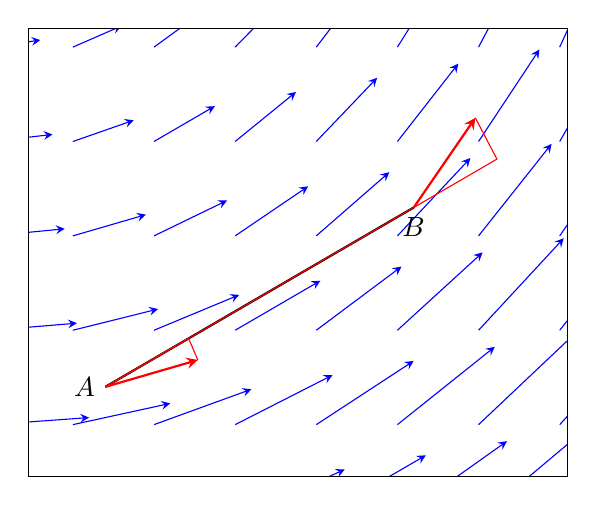
\begin{tikzpicture}
		\begin{axis}[xmin=0.5,xmax=4,ymin=0.5,ymax=3, view={0}{90},ticks=none]
			\addplot3[thin, blue, quiver={u={2.5-0.5*y}, v={0.5*x}, scale arrows=0.3}, -stealth,samples=20] {0};
			\coordinate (A) at (axis cs:1,1);
			\coordinate (Ma) at (axis cs:1.6,1.150);
			\coordinate (B) at (axis cs:3,2);
			\coordinate (Mb) at (axis cs:3.4,2.5);
			\draw[thick] (A) -- (B) node[pos=0,anchor=east]{$A$} node[pos=1,anchor=north]{$B$};
			\draw[thick,red,-stealth] (A) -- (Ma);
			\draw[thick,red,-stealth] (B) -- (Mb);
			\draw[red] (A) -- (axis cs: 1+0.27*2,1+0.27) -- (Ma);
			\draw[red] (A) -- (axis cs: 3+0.27*2,2+0.27) -- (Mb);
		\end{axis}
	\end{tikzpicture}
	\caption{Représentation d'un champ de vecteurs équiprojectif (flèches) : la projection sur le segment $AB$ de la valeur du champ en $A$ est identique à la projection sur ce même segment de la valeur du champ en $B$.}
	\label{fig:equiprojectivite}
\end{figure}

	\subsection{\'Elements de réduction d'un torseur}
	Un torseur est un object mathématique constitué :
	\begin{itemize}
		\item d'un vecteur, appelé résultante
		\item d'un champ de moment
	\end{itemize}
	
	Comme le champ de moment respecte la formule du champ de moment (voir ci-après), la connaissance de la valeur de ce champ en un point suffit à déterminer la valeur du champ en tout point de l'espace. Soient \vect{R} la résultante et $\vect{M}_A$ le moment en $A$ du torseur $\lbrace\mathcal{T}\rbrace$. Ce dernier peut alors s'écrire sous la forme suivante :
	\begin{equation}
		\left\lbrace\mathcal{T}\right\rbrace=\left\lbrace\begin{array}{c}
			\vect{R}\\
			\vect{M}_A
		\end{array}\right\rbrace_A
	\end{equation}
	\vect{R} et $\vect{M}_A$ sont les éléments de réduction du torseur.
	
	\subsection{Champ de moments de torseur}
		\label{sec:champ-de-moments}
		La valeur du moment en tout point $B$ de l'espace $E$, notée $\vect{M}_B$, peut se calculer ainsi :
		\begin{equation}
			\label{eq:champ-de-moments}
			\forall B\in E \quad \vect{M}_B=\vect{M}_A+\vect{BA}\wedge\vect{R}
		\end{equation}
		
	\subsection{Axe central d'un torseur}
		\label{sec:axe-central}
		On appelle axe central d'un torseur l'ensemble des points où la norme du moment est minimale. Cet axe est aussi caractérisé par le fait que résultante et moment y sont colinéaires.
		
		
	\subsection{Opérations entre torseurs}
		Soient deux torseurs $\lbrace\mathcal{T}\rbrace$ et $\lbrace\mathcal{T}'\rbrace$ avec :
		\begin{equation}
			\left\lbrace\mathcal{T}\right\rbrace=\left\lbrace\begin{array}{c}
				\vect{R}\\
				\vect{M}_A
			\end{array}\right\rbrace_A
			\quad
			\text{et}
			\quad
			\left\lbrace\mathcal{T}'\right\rbrace=\left\lbrace\begin{array}{c}
				\vect{R}'\\
				\vect{M}_A'
			\end{array}\right\rbrace_A					
		\end{equation}

		\subsubsection{Somme}
		La somme de deux torseurs se calcule comme la somme de ses éléments de réduction, calculés en un même point :
		\begin{equation}
			\left\lbrace\mathcal{T}\right\rbrace+\left\lbrace\mathcal{T}'\right\rbrace=
			\left\lbrace\begin{array}{c}
				\vect{R}+\vect{R}'\\
				\vect{M}_A+\vect{M}_A'
			\end{array}\right\rbrace_A			
		\end{equation}
		
		\subsubsection{Produit}
			\label{sec:produit-torseurs}
		Le produit de deux torseurs se calcule comme la somme des produits croisés de leurs éléments de réduction, calculés en un même point :
		\begin{equation}
			\left\lbrace\mathcal{T}\right\rbrace\cdot\left\lbrace\mathcal{T}'\right\rbrace=
				\vect{R}\cdot\vect{M}_A'+\vect{M}_A\cdot\vect{R}'
		\end{equation}
		Cette somme est indépendante du point auquel sont calculés les moments.	
		
		\subsubsection{Égalité}
		Deux torseurs sont égaux si et seulement si leurs éléments de réductions, calculés au même point, sont égaux deux à deux :
		\begin{equation}
			\left\lbrace\mathcal{T}\right\rbrace=\left\lbrace\mathcal{T}'\right\rbrace
			\quad\Leftrightarrow\quad
			\left\lbrace
				\begin{aligned}
					\vect{R}&=\vect{R}'\\
					\vect{M}_A&=\vect{M}_A'
				\end{aligned}
			\right\rbrace
		\end{equation}	
		

